\documentclass{article}%
\usepackage[T1]{fontenc}%
\usepackage[utf8]{inputenc}%
\usepackage{lmodern}%
\usepackage{textcomp}%
\usepackage{lastpage}%
\usepackage{geometry}%
\geometry{landscape=True,margin=0.5in,headheight=20pt,headsep=10pt,includeheadfoot=True}%
\usepackage{longtable}%
\usepackage{tabu}%
%
\usepackage{geometry}
\usepackage{xcolor}
\usepackage{amsmath}
\usepackage[some]{background}
\usepackage{lipsum}
\usepackage{color}%
\usepackage{hyperref}
\usepackage{tikz}%
\definecolor{titlepagecolor}{cmyk}{1,.60,0,.40}
\usepackage{float}

\DeclareFixedFont{\bigsf}{T1}{phv}{b}{n}{1.5cm}

\backgroundsetup{
scale=1,
angle=0,
opacity=1,
contents={\begin{tikzpicture}[remember picture,overlay]
 \path [fill=titlepagecolor] (-0.5\paperwidth,5) rectangle (0.5\paperwidth,10);
\end{tikzpicture}}
}
\author{%
    MD EIMRAN HOSSAIN EIMON \\
    \texttt{mdeimranhossaineimon@gmail.com}\vspace{40pt} \\

    }
\makeatletter
\def\printauthor{%
    {\large \@author}}
\makeatother


\hypersetup{
    colorlinks=true, %set true if you want colored links
    linktoc=all,     %set to all if you want both sections and subsections linked
    linkcolor=blue,  %choose some color if you want links to stand out
}
%
\usepackage{fancyhdr}%
\renewcommand{\headrulewidth}{0pt}%
\author{Md Eimran Hossain Eimon\newline%
 mdeimranhossaineimon@gmail.com}%
%
\begin{document}%
\normalsize%
\begin{titlepage}
\BgThispage
\newgeometry{left=1cm,right=4cm}
\noindent
\textcolor{white}{\bigsf Complexity \& Power Analysis}
\vspace*{2.5cm}\par
\noindent
\begin{minipage}{0.35\linewidth}
    \begin{flushright}
        \printauthor
    \end{flushright}
\end{minipage} \hspace{15pt}
%
\begin{minipage}{0.02\linewidth}
    \rule{2pt}{275pt}
\end{minipage} \hspace{-10pt}
%
\begin{minipage}{0.6\linewidth}
\vspace{5pt}

{\huge An abstract is a brief summary of a research article, thesis, review, conference proceeding or any in-depth analysis of a particular subject or discipline, and is often used to help.}

\end{minipage}
\end{titlepage}

\restoregeometry%%
\tableofcontents%
\pagestyle{fancy}%
\fancyhf{}%
\fancyhead[L]{\rightmark}%
\fancyhead[R]{\thepage}%
\newpage%
\section{Analysis Summary}%
\label{sec:AnalysisSummary}%
\subsection{Encoding Summary}%
\label{subsec:EncodingSummary}%
\begin{longtabu}{| X[l] | X[l] | X[l] | X[l] | X[l] |}%
\caption{%
Encoding Combination Used%
}%
\hline%
&&&&\\%
\textbf{Combination No.}&\textbf{Seq Name}&\textbf{Codec Name}&\textbf{Config Name}&\textbf{QP}\\%
&&&&\\%
\hline%
\endhead%
1&{[}'RaceHorses\_416x240\_30'{]}&hm&encoder\_lowdelay\_main&22\\%
\hline%
2&{[}'RaceHorses\_416x240\_30'{]}&hm&encoder\_lowdelay\_main&27\\%
\hline%
3&{[}'RaceHorses\_416x240\_30'{]}&hm&encoder\_lowdelay\_main&32\\%
\hline%
4&{[}'RaceHorses\_416x240\_30'{]}&hm&encoder\_lowdelay\_main&37\\%
\hline%
\end{longtabu}%
\begin{longtabu}{| X[l] | X[l] | X[l] | X[l] | X[l] |}%
\caption{%
Encoding Results%
}%
\hline%
&&&&\\%
\textbf{Combination No.}&\textbf{Bitrate}&\textbf{Y{-}PSNR}&\textbf{CPU Time}&\textbf{Enc\_FPS/FR}\\%
&&&&\\%
\hline%
\endhead%
1&3428.7600&41.0101&3.290s&0.02\\%
\hline%
2&2044.8000&36.8827&2.130s&0.031\\%
\hline%
3&1188.9600&33.2687&2.220s&0.03\\%
\hline%
4&627.9600&30.0505&1.360s&0.049\\%
\hline%
\end{longtabu}

%
\newpage%
\subsection{Decoding Summary}%
\label{subsec:DecodingSummary}%
\begin{longtabu}{| X[l] | X[l] | X[l] | X[l] |}%
\caption{%
Decoding Combination Used%
}%
\hline%
&&&\\%
\textbf{Combination No.}&\textbf{Seq}&\textbf{Codec}&\textbf{Cfg}\\%
&&&\\%
\hline%
\endhead%
1&RaceHorses\_416x240\_30\_QP\_22&hm&encoder\_lowdelay\_main.cfg\\%
\hline%
2&RaceHorses\_416x240\_30\_QP\_27&hm&encoder\_lowdelay\_main.cfg\\%
\hline%
3&RaceHorses\_416x240\_30\_QP\_32&hm&encoder\_lowdelay\_main.cfg\\%
\hline%
4&RaceHorses\_416x240\_30\_QP\_37&hm&encoder\_lowdelay\_main.cfg\\%
\hline%
\end{longtabu}%
\begin{longtabu}{| X[l] | X[l] | X[l] | X[l] | X[l] |}%
\caption{%
Decoding Results%
}%
\hline%
&&&&\\%
\textbf{Combination No.}&\textbf{Bitrate (kbps)}&\textbf{CPU Time}&\textbf{ Average Power (mW)}&\textbf{Total Energy (mJ)}\\%
&&&&\\%
\hline%
\endhead%
1&3428.7600&0.020s&5363.03&193.12\\%
\hline%
2&2044.8000&0.040s&10953.05&197.57\\%
\hline%
3&1188.9600&0.030s&6924.34&174.5\\%
\hline%
4&627.9600&0.030s&5250.44&111.76\\%
\hline%
\end{longtabu}

%
\newpage%
\section{Complexity Analysis {-} (Codec Name: HM)}%
\label{sec:ComplexityAnalysis{-}(CodecNameHM)}%
\subsection{HM ENCODER's Complexity}%
\label{subsec:HMENCODERsComplexity}%
\begin{figure}[H] \centering{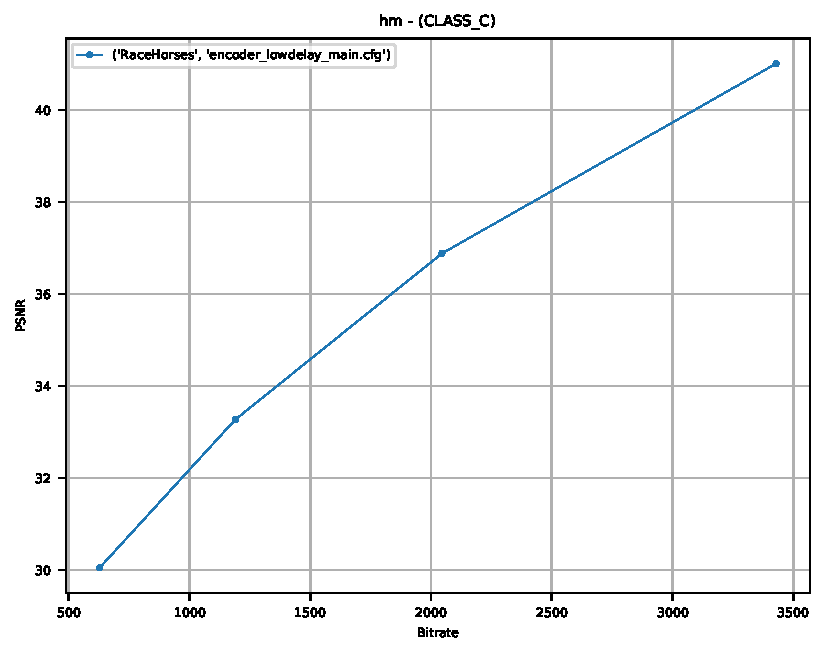
\includegraphics[scale=1.2]{%
/home/ridi/Desktop/Research_VVC_HM/results_2021_04_19_02_36_13/hm/encoder/hm_CLASS_C.pdf%
}}\end{figure}%
\newpage%
\subsubsection{Config Name: encoder\_lowdelay\_main.cfg, Class Name: CLASS\_C}%
\label{ssubsec:ConfigNameencoderlowdelaymain.cfg,ClassNameCLASSC}%
\begin{longtabu}{| X[l] | X[l] |}%
\caption{%
Hotpots By Class (RaceHorses, QP =22)%
}%
\hline%
&\\%
\textbf{Class}&\textbf{CPU Time (\%)}\\%
&\\%
\hline%
\endhead%
xRateDistOptQuant&27.599\\%
\hline%
codeCoeffNxN&8.693\\%
\hline%
getSigCtxInc&4.621\\%
\hline%
encodeBin&2.675\\%
\hline%
&\\%
\hline%
xEstimateInterResidualQT&2.432\\%
\hline%
estBit&2.067\\%
\hline%
xPredIntraAng&2.067\\%
\hline%
filter<(int)8, (bool)0, (bool)1, (bool)0>&1.824\\%
\hline%
&\\%
\hline%
xIntraCodingTUBlock&1.824\\%
\hline%
xCalcHADs4x4&1.58\\%
\hline%
xGetSAD8&1.216\\%
\hline%
filter<(int)8, (bool)1, (bool)0, (bool)1>&1.216\\%
\hline%
&\\%
\hline%
xGetExpGolombNumberOfBits&1.216\\%
\hline%
resetBits&1.094\\%
\hline%
xGetSSE32&0.973\\%
\hline%
estIntraPredLumaQT&0.973\\%
\hline%
&\\%
\hline%
xGetSSE8&0.973\\%
\hline%
xWriteCoefRemainExGolomb&0.972\\%
\hline%
getIntraDirPredictor&0.73\\%
\hline%
estSignificantMapBit&0.73\\%
\hline%
\end{longtabu}%
\newpage%
\begin{longtabu}{| X[l] | X[l] |}%
\caption{%
Hotspots By Function\newline%
 Config Name: encoder\_lowdelay\_main.cfg,\newline%
 Class Name: CLASS\_C\newline%
 (RaceHorses, QP =22)%
}%
\hline%
&\\%
\textbf{Function}&\textbf{CPU Time}\\%
&\\%
\hline%
\endhead%
TComTrQuant::xRateDistOptQuant&0.908015\\%
\hline%
TEncSbac::codeCoeffNxN&0.285994\\%
\hline%
TComTrQuant::getSigCtxInc&0.152019\\%
\hline%
\_\_memmove\_avx\_unaligned\_erms&0.107963\\%
\hline%
&\\%
\hline%
\_\_memset\_avx2\_unaligned\_erms&0.104025\\%
\hline%
TEncBinCABACCounter::encodeBin&0.087996\\%
\hline%
TEncSearch::xEstimateInterResidualQT&0.080001\\%
\hline%
TEncSbac::estBit&0.068002\\%
\hline%
&\\%
\hline%
TComPrediction::xPredIntraAng&0.067992\\%
\hline%
TComInterpolationFilter::filter<(int)8, (bool)0, (bool)1, (bool)0>&0.060003\\%
\hline%
TEncSearch::xIntraCodingTUBlock&0.059998\\%
\hline%
TComRdCost::xCalcHADs4x4&0.051996\\%
\hline%
&\\%
\hline%
\_Z15simd8x8HAD1D32bPDv2\_xS0\_&0.047994\\%
\hline%
simdHADs8x8&0.043996\\%
\hline%
TComRdCost::xGetSAD8&0.040011\\%
\hline%
TComInterpolationFilter::filter<(int)8, (bool)1, (bool)0, (bool)1>&0.039999\\%
\hline%
&\\%
\hline%
TComRdCost::xGetExpGolombNumberOfBits&0.039999\\%
\hline%
TComRdCost::xGetSSE32&0.032021\\%
\hline%
TEncSearch::estIntraPredLumaQT&0.032000\\%
\hline%
TComRdCost::xGetSSE8&0.031996\\%
\hline%
\end{longtabu}%
\newpage%
\begin{longtabu}{| X[l] | X[l] |}%
\caption{%
Memory Consumption\newline%
 Config Name: encoder\_lowdelay\_main.cfg,\newline%
 Class Name: CLASS\_C\newline%
 (RaceHorses, QP =22)%
}%
\hline%
&\\%
\textbf{Function}&\textbf{Allocation/Deallocation Delta}\\%
&\\%
\hline%
\endhead%
func@0x8f3f0&72704.000000\\%
\hline%
main&4096.000000\\%
\hline%
\_\_libc\_csu\_init&1040.000000\\%
\hline%
\_\_static\_initialization\_and\_destruction\_0.constprop.69&1040.000000\\%
\hline%
&\\%
\hline%
EnvVar::EnvVar&690.000000\\%
\hline%
\_\_register\_frame&480.000000\\%
\hline%
\_GLOBAL\_\_sub\_I\_\_ZN3SEI19prefix\_sei\_messagesE&212.000000\\%
\hline%
indentNewLines&210.000000\\%
\hline%
&\\%
\hline%
TAppEncCfg::parseCfg&0.0\\%
\hline%
TAppEncCfg::xCheckParameter&0.0\\%
\hline%
TAppEncTop::encode&0.0\\%
\hline%
TAppEncTop::xGetBuffer&0.0\\%
\hline%
&\\%
\hline%
TComCUMvField::create&0.0\\%
\hline%
TComDataCU::create&0.0\\%
\hline%
TComLoopFilter::create&0.0\\%
\hline%
TComOutputBitstream::addSubstream&0.0\\%
\hline%
&\\%
\hline%
TComOutputBitstream::write&0.0\\%
\hline%
TComPic::create&0.0\\%
\hline%
TComPic::prepareForReconstruction&0.0\\%
\hline%
TComPicSym::TComPicSym&0.0\\%
\hline%
\end{longtabu}%
\newpage%
\begin{longtabu}{| X[l] | X[l] | X[l] | X[l] | X[l] | X[l] | X[l] |}%
\caption{%
Performance Snapshot\newline%
 Config Name: encoder\_lowdelay\_main.cfg,\newline%
 Class Name: CLASS\_C\newline%
%
}%
\hline%
&&&&&&\\%
\textbf{Seq Name}&\textbf{Elapsed Time}&\textbf{IPC}&\textbf{Effective Logical Core Utilization}&\textbf{Effective Physical Core Utilization}&\textbf{Microarchitecture Usage}&\textbf{GPU Active Time}\\%
&&&&&&\\%
\hline%
\endhead%
RaceHorses\newline%
 QP = qp&2.141s&2.183&14.4\% (1.150 out of 8)&27.6\% (1.105 out of 4)&56.5\% of Pipeline Slots&1.2\%\\%
\hline%
RaceHorses\newline%
 QP = qp&1.933s&2.128&14.1\% (1.132 out of 8)&27.8\% (1.113 out of 4)&55.1\% of Pipeline Slots&1.3\%\\%
\hline%
RaceHorses\newline%
 QP = qp&1.413s&2.253&14.6\% (1.171 out of 8)&28.7\% (1.147 out of 4)&59.9\% of Pipeline Slots&0.6\%\\%
\hline%
RaceHorses\newline%
 QP = qp&2.854s&2.004&13.9\% (1.109 out of 8)&26.6\% (1.064 out of 4)&53.9\% of Pipeline Slots&1.2\%\\%
\hline%
\end{longtabu}%
\begin{longtabu}{| X[l] | X[l] | X[l] | X[l] | X[l] | X[l] | X[l] | X[l] |}%
\caption{%
Instruction Mix\newline%
 Config Name: encoder\_lowdelay\_main.cfg,\newline%
 Class Name: CLASS\_C\newline%
%
}%
\hline%
&&&&&&&\\%
\textbf{Seq Name}&\textbf{Elapsed Time}&\textbf{SP FLOPs}&\textbf{DP FLOPs}&\textbf{x87 FLOPs}&\textbf{Non{-}FP}&\textbf{FP Arith/Mem Rd Instr. Ratio}&\textbf{FP Arith/Mem Wr Instr. Ratio}\\%
&&&&&&&\\%
\hline%
\endhead%
RaceHorses\newline%
 QP = qp&2.141s&0.0\% of uOps&1.2\% of uOps&0.1\% of uOps&98.8\% of uOps&0.044&0.100\\%
\hline%
RaceHorses\newline%
 QP = qp&1.933s&0.0\% of uOps&1.2\% of uOps&0.1\% of uOps&98.8\% of uOps&0.045&0.100\\%
\hline%
RaceHorses\newline%
 QP = qp&1.413s&0.0\% of uOps&1.1\% of uOps&0.1\% of uOps&98.8\% of uOps&0.042&0.095\\%
\hline%
RaceHorses\newline%
 QP = qp&2.854s&0.0\% of uOps&1.2\% of uOps&0.1\% of uOps&98.7\% of uOps&0.046&0.107\\%
\hline%
\end{longtabu}%
\newpage%
\begin{longtabu}{| X[l] | X[l] | X[l] | X[l] | X[l] | X[l] | X[l] |}%
\caption{%
GPU Usage\newline%
 Config Name: encoder\_lowdelay\_main.cfg,\newline%
 Class Name: CLASS\_C\newline%
%
}%
\hline%
&&&&&&\\%
\textbf{Seq Name}&\textbf{Elapsed Time}&\textbf{GPU Utilization when Busy}&\textbf{Active}&\textbf{Stalled}&\textbf{Idle}&\textbf{Occupancy}\\%
&&&&&&\\%
\hline%
\endhead%
RaceHorses\newline%
 QP = qp&2.141s&17.4\%&17.4\%&32.7\%&49.9\%&30.5\% of peak value\\%
\hline%
RaceHorses\newline%
 QP = qp&1.933s&22.1\%&22.1\%&33.9\%&44.0\%&36.2\% of peak value\\%
\hline%
RaceHorses\newline%
 QP = qp&1.413s&7.4\%&7.4\%&33.5\%&59.1\%&21.3\% of peak value\\%
\hline%
RaceHorses\newline%
 QP = qp&2.854s&16.8\%&16.8\%&30.2\%&53.0\%&28.8\% of peak value\\%
\hline%
\end{longtabu}%
\begin{longtabu}{| X[l] | X[l] | X[l] | X[l] | X[l] | X[l] | X[l] | X[l] | X[l] |}%
\caption{%
Memory Access Analysis\newline%
 Config Name: encoder\_lowdelay\_main.cfg,\newline%
 Class Name: CLASS\_C\newline%
%
}%
\hline%
&&&&&&&&\\%
\textbf{Seq Name}&\textbf{CPU Time}&\textbf{L1 Bound}&\textbf{L2 Bound}&\textbf{L3 Bound}&\textbf{DRAM Bound}&\textbf{Store Bound}&\textbf{LLC Miss Count}&\textbf{Average Latency (cycles)}\\%
&&&&&&&&\\%
\hline%
\endhead%
RaceHorses\newline%
 QP = qp&1.500s&5.5\% of Clockticks&0.5\% of Clockticks&0.5\% of Clockticks&0.0\% of Clockticks&1.4\% of Clockticks&0&9\\%
\hline%
RaceHorses\newline%
 QP = qp&3.013s&5.9\% of Clockticks&0.3\% of Clockticks&0.7\% of Clockticks&0.0\% of Clockticks&1.0\% of Clockticks&0&9\\%
\hline%
RaceHorses\newline%
 QP = qp&1.208s&4.5\% of Clockticks&0.6\% of Clockticks&0.6\% of Clockticks&0.0\% of Clockticks&1.7\% of Clockticks&0&10\\%
\hline%
RaceHorses\newline%
 QP = qp&3.044s&6.4\% of Clockticks&0.3\% of Clockticks&0.5\% of Clockticks&0.0\% of Clockticks&0.8\% of Clockticks&0&8\\%
\hline%
\end{longtabu}%
\newpage%
\begin{longtabu}{| X[l] | X[l] | X[l] | X[l] | X[l] | X[l] | X[l] | X[l] |}%
\caption{%
Micro Architecture Exploration\newline%
 Config Name: encoder\_lowdelay\_main.cfg,\newline%
 Class Name: CLASS\_C\newline%
%
}%
\hline%
&&&&&&&\\%
\textbf{Seq Name}&\textbf{Elapsed Time}&\textbf{Clockticks}&\textbf{Instructions Retired}&\textbf{CPI Rate}&\textbf{Bad Speculation}&\textbf{Branch Mispredict}&\textbf{Vector Capacity Usage (FPU)}\\%
&&&&&&&\\%
\hline%
\endhead%
RaceHorses\newline%
 QP = qp&2.593s&5,338,800,000&12,364,200,000&0.432&9.1\% of Pipeline Slots&9.1\% of Pipeline Slots&25.0\%\\%
\hline%
RaceHorses\newline%
 QP = qp&2.984s&6,807,600,000&15,359,400,000&0.443&12.5\% of Pipeline Slots&12.5\% of Pipeline Slots&25.0\%\\%
\hline%
RaceHorses\newline%
 QP = qp&1.277s&4,273,200,000&10,402,200,000&0.411&7.6\% of Pipeline Slots&7.6\% of Pipeline Slots&25.0\%\\%
\hline%
RaceHorses\newline%
 QP = qp&3.685s&9,318,600,000&20,179,800,000&0.462&14.1\% of Pipeline Slots&14.1\% of Pipeline Slots&25.0\%\\%
\hline%
\end{longtabu}%
\begin{longtabu}{| X[l] | X[l] | X[l] | X[l] | X[l] | X[l] | X[l] | X[l] |}%
\caption{%
Front{-}End Bound Analysis\newline%
 Config Name: encoder\_lowdelay\_main.cfg,\newline%
 Class Name: CLASS\_C\newline%
%
}%
\hline%
&&&&&&&\\%
\textbf{Seq Name}&\textbf{Elapsed Time}&\textbf{Front{-}End Bound}&\textbf{Front{-}End Latency}&\textbf{ICache Misses}&\textbf{ITLB Overhead}&\textbf{Branch Resteers}&\textbf{Front{-}End Bandwidth}\\%
&&&&&&&\\%
\hline%
\endhead%
RaceHorses\newline%
 QP = qp&2.593s&19.0\% of Pipeline Slots&7.1\% of Pipeline Slots&2.0\% of Clockticks&0.3\% of Clockticks&3.9\% of Clockticks&11.9\% of Pipeline Slots\\%
\hline%
RaceHorses\newline%
 QP = qp&2.984s&19.2\% of Pipeline Slots&8.1\% of Pipeline Slots&1.6\% of Clockticks&0.2\% of Clockticks&4.7\% of Clockticks&11.1\% of Pipeline Slots\\%
\hline%
RaceHorses\newline%
 QP = qp&1.277s&18.3\% of Pipeline Slots&6.3\% of Pipeline Slots&2.5\% of Clockticks&0.3\% of Clockticks&3.1\% of Clockticks&12.0\% of Pipeline Slots\\%
\hline%
RaceHorses\newline%
 QP = qp&3.685s&19.4\% of Pipeline Slots&8.1\% of Pipeline Slots&1.7\% of Clockticks&0.4\% of Clockticks&5.7\% of Clockticks&11.3\% of Pipeline Slots\\%
\hline%
\end{longtabu}%
\newpage%
\begin{longtabu}{| X[l] | X[l] | X[l] | X[l] | X[l] | X[l] | X[l] | X[l] | X[l] |}%
\caption{%
Back{-}End Bound Analysis\newline%
 Config Name: encoder\_lowdelay\_main.cfg,\newline%
 Class Name: CLASS\_C\newline%
%
}%
\hline%
&&&&&&&&\\%
\textbf{Seq Name}&\textbf{Elapsed Time}&\textbf{Back{-}End Bound}&\textbf{L1 Bound}&\textbf{L2 Bound}&\textbf{L3 Bound}&\textbf{DRAM Bound}&\textbf{Store Bound}&\textbf{Store Latency}\\%
&&&&&&&&\\%
\hline%
\endhead%
RaceHorses\newline%
 QP = qp&2.593s&9.5\% of Pipeline Slots&5.1\% of Clockticks&1.0\% of Clockticks&0.0\% of Clockticks&0.0\% of Clockticks&1.0\% of Clockticks&10.3\% of Clockticks\\%
\hline%
RaceHorses\newline%
 QP = qp&2.984s&8.2\% of Pipeline Slots&6.3\% of Clockticks&0.8\% of Clockticks&0.0\% of Clockticks&0.0\% of Clockticks&0.8\% of Clockticks&8.1\% of Clockticks\\%
\hline%
RaceHorses\newline%
 QP = qp&1.277s&11.9\% of Pipeline Slots&5.1\% of Clockticks&0.0\% of Clockticks&0.0\% of Clockticks&0.0\% of Clockticks&1.3\% of Clockticks&10.5\% of Clockticks\\%
\hline%
RaceHorses\newline%
 QP = qp&3.685s&11.6\% of Pipeline Slots&6.4\% of Clockticks&0.6\% of Clockticks&0.0\% of Clockticks&0.0\% of Clockticks&0.6\% of Clockticks&7.0\% of Clockticks\\%
\hline%
\end{longtabu}%
\newpage

%
\subsection{HM DECODER's Complexity}%
\label{subsec:HMDECODERsComplexity}%
\subsubsection{Config Name: encoder\_lowdelay\_main.cfg, Class Name: CLASS\_C}%
\label{ssubsec:ConfigNameencoderlowdelaymain.cfg,ClassNameCLASSC}%
\begin{longtabu}{| X[l] | X[l] |}%
\caption{%
Hotpots By Class (RaceHorses, QP =hm)%
}%
\hline%
&\\%
\textbf{Class}&\textbf{CPU Time (\%)}\\%
&\\%
\hline%
\endhead%
istream&369.815\\%
\hline%
decodeBinEP&100.01\\%
\hline%
decodeBin&50.115\\%
\hline%
parseQtCbf&50.0\\%
\hline%
&\\%
\hline%
xPredInterUni&40.005\\%
\hline%
\end{longtabu}%
\newpage%
\begin{longtabu}{| X[l] | X[l] |}%
\caption{%
Hotspots By Function\newline%
 Config Name: encoder\_lowdelay\_main.cfg,\newline%
 Class Name: CLASS\_C\newline%
 (RaceHorses, QP =hm)%
}%
\hline%
&\\%
\textbf{Function}&\textbf{CPU Time}\\%
&\\%
\hline%
\endhead%
std::istream::get&0.021999\\%
\hline%
TComPrediction::xPredInterUni&0.008001\\%
\hline%
Function&CPU Time\\%
\hline%
std::istream::get&0.019977\\%
\hline%
&\\%
\hline%
TDecBinCABAC::decodeBin&0.010023\\%
\hline%
TDecBinCABAC::decodeBinEP&0.010000\\%
\hline%
Function&CPU Time\\%
\hline%
std::istream::get&0.011987\\%
\hline%
&\\%
\hline%
TDecBinCABAC::decodeBinEP&0.010002\\%
\hline%
TDecSbac::parseQtCbf&0.010000\\%
\hline%
func@0x11350&0.008012\\%
\hline%
Function&CPU Time\\%
\hline%
&\\%
\hline%
std::istream::get&0.020000\\%
\hline%
\end{longtabu}%
\newpage%
\begin{longtabu}{| X[l] | X[l] |}%
\caption{%
Memory Consumption\newline%
 Config Name: encoder\_lowdelay\_main.cfg,\newline%
 Class Name: CLASS\_C\newline%
 (RaceHorses, QP =hm)%
}%
\hline%
&\\%
\textbf{Function}&\textbf{Allocation/Deallocation Delta}\\%
&\\%
\hline%
\endhead%
byteStreamNALUnit&350840.000000\\%
\hline%
func@0x8f3f0&72704.000000\\%
\hline%
main&4096.000000\\%
\hline%
\_\_libc\_csu\_init&1040.000000\\%
\hline%
&\\%
\hline%
\_\_register\_frame&480.000000\\%
\hline%
\_GLOBAL\_\_sub\_I\_\_ZN3SEI19prefix\_sei\_messagesE&212.000000\\%
\hline%
TAppDecCfg::parseCfg&0.0\\%
\hline%
TAppDecTop::decode&0.0\\%
\hline%
&\\%
\hline%
TComCUMvField::create&0.0\\%
\hline%
TComDataCU::create&0.0\\%
\hline%
TComInputBitstream::extractSubstream&0.0\\%
\hline%
TComLoopFilter::create&0.0\\%
\hline%
&\\%
\hline%
TComPic::create&0.0\\%
\hline%
TComPicSym::TComPicSym&0.0\\%
\hline%
TComPicSym::allocateNewSlice&0.0\\%
\hline%
TComPicSym::create&0.0\\%
\hline%
&\\%
\hline%
TComPicSym::prepareForReconstruction&0.0\\%
\hline%
TComPicSym::xInitTiles&0.0\\%
\hline%
TComPicYuv::create&0.0\\%
\hline%
TComPicYuv::createWithoutCUInfo&0.0\\%
\hline%
\end{longtabu}%
\newpage%
\begin{longtabu}{| X[l] | X[l] | X[l] | X[l] | X[l] | X[l] | X[l] |}%
\caption{%
Performance Snapshot\newline%
 Config Name: encoder\_lowdelay\_main.cfg,\newline%
 Class Name: CLASS\_C\newline%
%
}%
\hline%
&&&&&&\\%
\textbf{Seq Name}&\textbf{Elapsed Time}&\textbf{IPC}&\textbf{Effective Logical Core Utilization}&\textbf{Effective Physical Core Utilization}&\textbf{Microarchitecture Usage}&\textbf{GPU Active Time}\\%
&&&&&&\\%
\hline%
\endhead%
RaceHorses\newline%
 QP = 32&0.048s&1.764&51.5\% (4.119 out of 8)&93.3\% (3.733 out of 4)&7.5\% of Pipeline Slots&4.9\%\\%
\hline%
RaceHorses\newline%
 QP = 37&0.044s&1.779&43.6\% (3.487 out of 8)&76.1\% (3.042 out of 4)&8.1\% of Pipeline Slots&47.2\%\\%
\hline%
RaceHorses\newline%
 QP = 22&0.078s&0.335&73.0\% (5.838 out of 8)&100.0\% (4.000 out of 4)&13.2\% of Pipeline Slots&18.2\%\\%
\hline%
RaceHorses\newline%
 QP = 27&0.053s&1.781&31.1\% (2.488 out of 8)&59.1\% (2.363 out of 4)&8.2\% of Pipeline Slots&4.4\%\\%
\hline%
\end{longtabu}%
\begin{longtabu}{| X[l] | X[l] | X[l] | X[l] | X[l] | X[l] | X[l] | X[l] |}%
\caption{%
Instruction Mix\newline%
 Config Name: encoder\_lowdelay\_main.cfg,\newline%
 Class Name: CLASS\_C\newline%
%
}%
\hline%
&&&&&&&\\%
\textbf{Seq Name}&\textbf{Elapsed Time}&\textbf{SP FLOPs}&\textbf{DP FLOPs}&\textbf{x87 FLOPs}&\textbf{Non{-}FP}&\textbf{FP Arith/Mem Rd Instr. Ratio}&\textbf{FP Arith/Mem Wr Instr. Ratio}\\%
&&&&&&&\\%
\hline%
\endhead%
RaceHorses\newline%
 QP = 32&0.048s&0.2\% of uOps&0.5\% of uOps&0.1\% of uOps&99.3\% of uOps&0.005&0.014\\%
\hline%
RaceHorses\newline%
 QP = 37&0.044s&0.2\% of uOps&0.5\% of uOps&0.1\% of uOps&99.2\% of uOps&0.011&0.031\\%
\hline%
RaceHorses\newline%
 QP = 22&0.078s&0.1\% of uOps&0.1\% of uOps&0.0\% of uOps&99.8\% of uOps&0.007&0.015\\%
\hline%
RaceHorses\newline%
 QP = 27&0.053s&0.2\% of uOps&0.5\% of uOps&0.1\% of uOps&99.1\% of uOps&0.004&0.011\\%
\hline%
\end{longtabu}%
\newpage%
\begin{longtabu}{| X[l] | X[l] | X[l] | X[l] | X[l] | X[l] | X[l] |}%
\caption{%
GPU Usage\newline%
 Config Name: encoder\_lowdelay\_main.cfg,\newline%
 Class Name: CLASS\_C\newline%
%
}%
\hline%
&&&&&&\\%
\textbf{Seq Name}&\textbf{Elapsed Time}&\textbf{GPU Utilization when Busy}&\textbf{Active}&\textbf{Stalled}&\textbf{Idle}&\textbf{Occupancy}\\%
&&&&&&\\%
\hline%
\endhead%
RaceHorses\newline%
 QP = 32&0.048s&39.5\%&39.5\%&23.9\%&36.6\%&47.6\% of peak value\\%
\hline%
RaceHorses\newline%
 QP = 37&0.044s&25.5\%&25.5\%&12.6\%&61.9\%&30.4\% of peak value\\%
\hline%
RaceHorses\newline%
 QP = 22&0.078s&35.4\%&35.4\%&15.0\%&49.6\%&41.9\% of peak value\\%
\hline%
RaceHorses\newline%
 QP = 27&0.053s&39.8\%&39.8\%&24.1\%&36.2\%&47.9\% of peak value\\%
\hline%
\end{longtabu}%
\begin{longtabu}{| X[l] | X[l] | X[l] | X[l] | X[l] | X[l] | X[l] | X[l] | X[l] |}%
\caption{%
Memory Access Analysis\newline%
 Config Name: encoder\_lowdelay\_main.cfg,\newline%
 Class Name: CLASS\_C\newline%
%
}%
\hline%
&&&&&&&&\\%
\textbf{Seq Name}&\textbf{CPU Time}&\textbf{L1 Bound}&\textbf{L2 Bound}&\textbf{L3 Bound}&\textbf{DRAM Bound}&\textbf{Store Bound}&\textbf{LLC Miss Count}&\textbf{Average Latency (cycles)}\\%
&&&&&&&&\\%
\hline%
\endhead%
RaceHorses\newline%
 QP = 32&0.038s&4.6\% of Clockticks&4.6\% of Clockticks&4.6\% of Clockticks&0.0\% of Clockticks&0.0\% of Clockticks&0&10\\%
\hline%
RaceHorses\newline%
 QP = 37&0.036s&5.8\% of Clockticks&0.0\% of Clockticks&5.8\% of Clockticks&0.0\% of Clockticks&0.0\% of Clockticks&0&7\\%
\hline%
RaceHorses\newline%
 QP = 22&0.027s&6.2\% of Clockticks&3.1\% of Clockticks&0.0\% of Clockticks&3.1\% of Clockticks&0.0\% of Clockticks&0&8\\%
\hline%
RaceHorses\newline%
 QP = 27&0.044s&8.0\% of Clockticks&0.0\% of Clockticks&0.0\% of Clockticks&4.0\% of Clockticks&0.0\% of Clockticks&0&8\\%
\hline%
\end{longtabu}%
\newpage%
\begin{longtabu}{| X[l] | X[l] | X[l] | X[l] | X[l] | X[l] | X[l] | X[l] |}%
\caption{%
Micro Architecture Exploration\newline%
 Config Name: encoder\_lowdelay\_main.cfg,\newline%
 Class Name: CLASS\_C\newline%
%
}%
\hline%
&&&&&&&\\%
\textbf{Seq Name}&\textbf{Elapsed Time}&\textbf{Clockticks}&\textbf{Instructions Retired}&\textbf{CPI Rate}&\textbf{Bad Speculation}&\textbf{Branch Mispredict}&\textbf{Vector Capacity Usage (FPU)}\\%
&&&&&&&\\%
\hline%
\endhead%
RaceHorses\newline%
 QP = 32&0.046s&49,140,000&76,500,000&0.642&8.2\% of Pipeline Slots&0.0\% of Pipeline Slots&0.0\%\\%
\hline%
RaceHorses\newline%
 QP = 37&0.045s&44,280,000&64,440,000&0.687&7.0\% of Pipeline Slots&0.0\% of Pipeline Slots&0.0\%\\%
\hline%
RaceHorses\newline%
 QP = 22&0.060s&70,020,000&112,320,000&0.623&11.6\% of Pipeline Slots&0.0\% of Pipeline Slots&0.0\%\\%
\hline%
RaceHorses\newline%
 QP = 27&0.052s&62,280,000&93,780,000&0.664&11.6\% of Pipeline Slots&0.0\% of Pipeline Slots&0.0\%\\%
\hline%
\end{longtabu}%
\begin{longtabu}{| X[l] | X[l] | X[l] | X[l] | X[l] | X[l] | X[l] | X[l] |}%
\caption{%
Front{-}End Bound Analysis\newline%
 Config Name: encoder\_lowdelay\_main.cfg,\newline%
 Class Name: CLASS\_C\newline%
%
}%
\hline%
&&&&&&&\\%
\textbf{Seq Name}&\textbf{Elapsed Time}&\textbf{Front{-}End Bound}&\textbf{Front{-}End Latency}&\textbf{ICache Misses}&\textbf{ITLB Overhead}&\textbf{Branch Resteers}&\textbf{Front{-}End Bandwidth}\\%
&&&&&&&\\%
\hline%
\endhead%
RaceHorses\newline%
 QP = 32&0.046s&24.7\% of Pipeline Slots&22.0\% of Pipeline Slots&11.0\% of Clockticks&0.0\% of Clockticks&0.0\% of Clockticks&2.7\% of Pipeline Slots\\%
\hline%
RaceHorses\newline%
 QP = 37&0.045s&27.9\% of Pipeline Slots&13.9\% of Pipeline Slots&0.0\% of Clockticks&1.2\% of Clockticks&12.2\% of Clockticks&13.9\% of Pipeline Slots\\%
\hline%
RaceHorses\newline%
 QP = 22&0.060s&19.3\% of Pipeline Slots&7.7\% of Pipeline Slots&7.7\% of Clockticks&0.8\% of Clockticks&7.7\% of Clockticks&11.6\% of Pipeline Slots\\%
\hline%
RaceHorses\newline%
 QP = 27&0.052s&28.9\% of Pipeline Slots&23.1\% of Pipeline Slots&0.0\% of Clockticks&0.9\% of Clockticks&0.0\% of Clockticks&5.8\% of Pipeline Slots\\%
\hline%
\end{longtabu}%
\newpage%
\begin{longtabu}{| X[l] | X[l] | X[l] | X[l] | X[l] | X[l] | X[l] | X[l] | X[l] |}%
\caption{%
Back{-}End Bound Analysis\newline%
 Config Name: encoder\_lowdelay\_main.cfg,\newline%
 Class Name: CLASS\_C\newline%
%
}%
\hline%
&&&&&&&&\\%
\textbf{Seq Name}&\textbf{Elapsed Time}&\textbf{Back{-}End Bound}&\textbf{L1 Bound}&\textbf{L2 Bound}&\textbf{L3 Bound}&\textbf{DRAM Bound}&\textbf{Store Bound}&\textbf{Store Latency}\\%
&&&&&&&&\\%
\hline%
\endhead%
RaceHorses\newline%
 QP = 32&0.046s&20.3\% of Pipeline Slots&0.0\% of Clockticks&0.0\% of Clockticks&0.0\% of Clockticks&11.0\% of Clockticks&0.0\% of Clockticks&0.0\% of Clockticks\\%
\hline%
RaceHorses\newline%
 QP = 37&0.045s&9.4\% of Pipeline Slots&24.4\% of Clockticks&0.0\% of Clockticks&0.0\% of Clockticks&0.0\% of Clockticks&0.0\% of Clockticks&0.0\% of Clockticks\\%
\hline%
RaceHorses\newline%
 QP = 22&0.060s&26.7\% of Pipeline Slots&7.7\% of Clockticks&0.0\% of Clockticks&0.0\% of Clockticks&0.0\% of Clockticks&0.0\% of Clockticks&0.0\% of Clockticks\\%
\hline%
RaceHorses\newline%
 QP = 27&0.052s&7.5\% of Pipeline Slots&8.7\% of Clockticks&0.0\% of Clockticks&8.7\% of Clockticks&8.7\% of Clockticks&0.0\% of Clockticks&8.7\% of Clockticks\\%
\hline%
\end{longtabu}%
\newpage

%
\end{document}